\documentclass[UTF8]{ctexart}

\usepackage{amsmath}
\usepackage{multicol}
\setlength{\parindent}{2em}
\addtolength{\topmargin}{-54pt}
\setlength{\oddsidemargin}{0.63cm}  % 3.17cm - 1 inch
\setlength{\evensidemargin}{\oddsidemargin}
\setlength{\textwidth}{14.66cm}
\setlength{\textheight}{24.00cm}    % 24.62
\usepackage{graphicx}
\usepackage{float}
\usepackage{multirow}
\usepackage{subfigure}
\usepackage{multirow}
\begin{document}

%标题
\begin{center}
\Huge\textbf{光纤光学与音频信号通信}
\renewcommand{\baselinestretch}{5.0}
\end{center}
\begin{center}
\small
\begin{tabular}{llll}
\textbf{姓名}&李励玮     &\textbf{学号}  &201711140236\\
\textbf{指导老师}&何娟琛 &\textbf{实验日期}& 2019.12.27\\
\end{tabular}
\end{center}

%摘要
\small
\noindent\textbf{摘要}:实验使用He-Ne激光器、光功率计、显微物镜、五维调整架、光纤、光纤切割刀、光纤错。分别测量了塑料光纤的损耗特性、商用光纤的数值孔径和二者的耦合效率,其中塑料光纤的耦合效率较高;而后利用光纤作为温度传感器,观察到了温度变化时,两束光相位差引起的干涉条纹移动,测量了干涉条纹变化数和温度之间的关系,得到了变化数-温差曲线。
\newline\textbf{关键字:光纤、耦合效率、损耗特性、数值孔径、光纤温度传感器}

\begin{multicols}{2}
%引言
\section{引言}
\subsection{定义}
光纤是光导纤维的简称。它是工作在光波波段的一种介质波导,利用光学全反射原理,将光的能量约束在光吸收和光散射都非常小的波导界面内,并引导光波沿着光纤轴线方向传播。

\subsection{应用}
现代信息社会得以实现的最重要的两大关键技术是激光和光纤。光纤通信具有通信容量大、传输距离远信号串扰小、保密性能好;抗电磁干扰、传输质量佳;光纤尺寸小、重量轻,便于敷设和运输;材料来源丰富,节约了大量有色金属铜;耐化学腐蚀,光缆适应性强,寿命长的特点。

光纤除了在现代通信系统的应用外,还应用于在传感器技术。光纤传感器是利用待测物理量对光纤内传输的光波的光学参量进行调制并传输至光学探测器进行解调,从而获得待测物理量的变化信息的装置,它具有损耗低、信息量大、线径细、质量轻可绕性好的特点,可用于位移、振动、压力、电流、磁场、温度、浓度等各种物理量的测量。
\subsection{结构}
光纤主要由纤芯、包层、涂敷层及套塑四部分组成,如图1。
\begin{figure}[H]
\centering
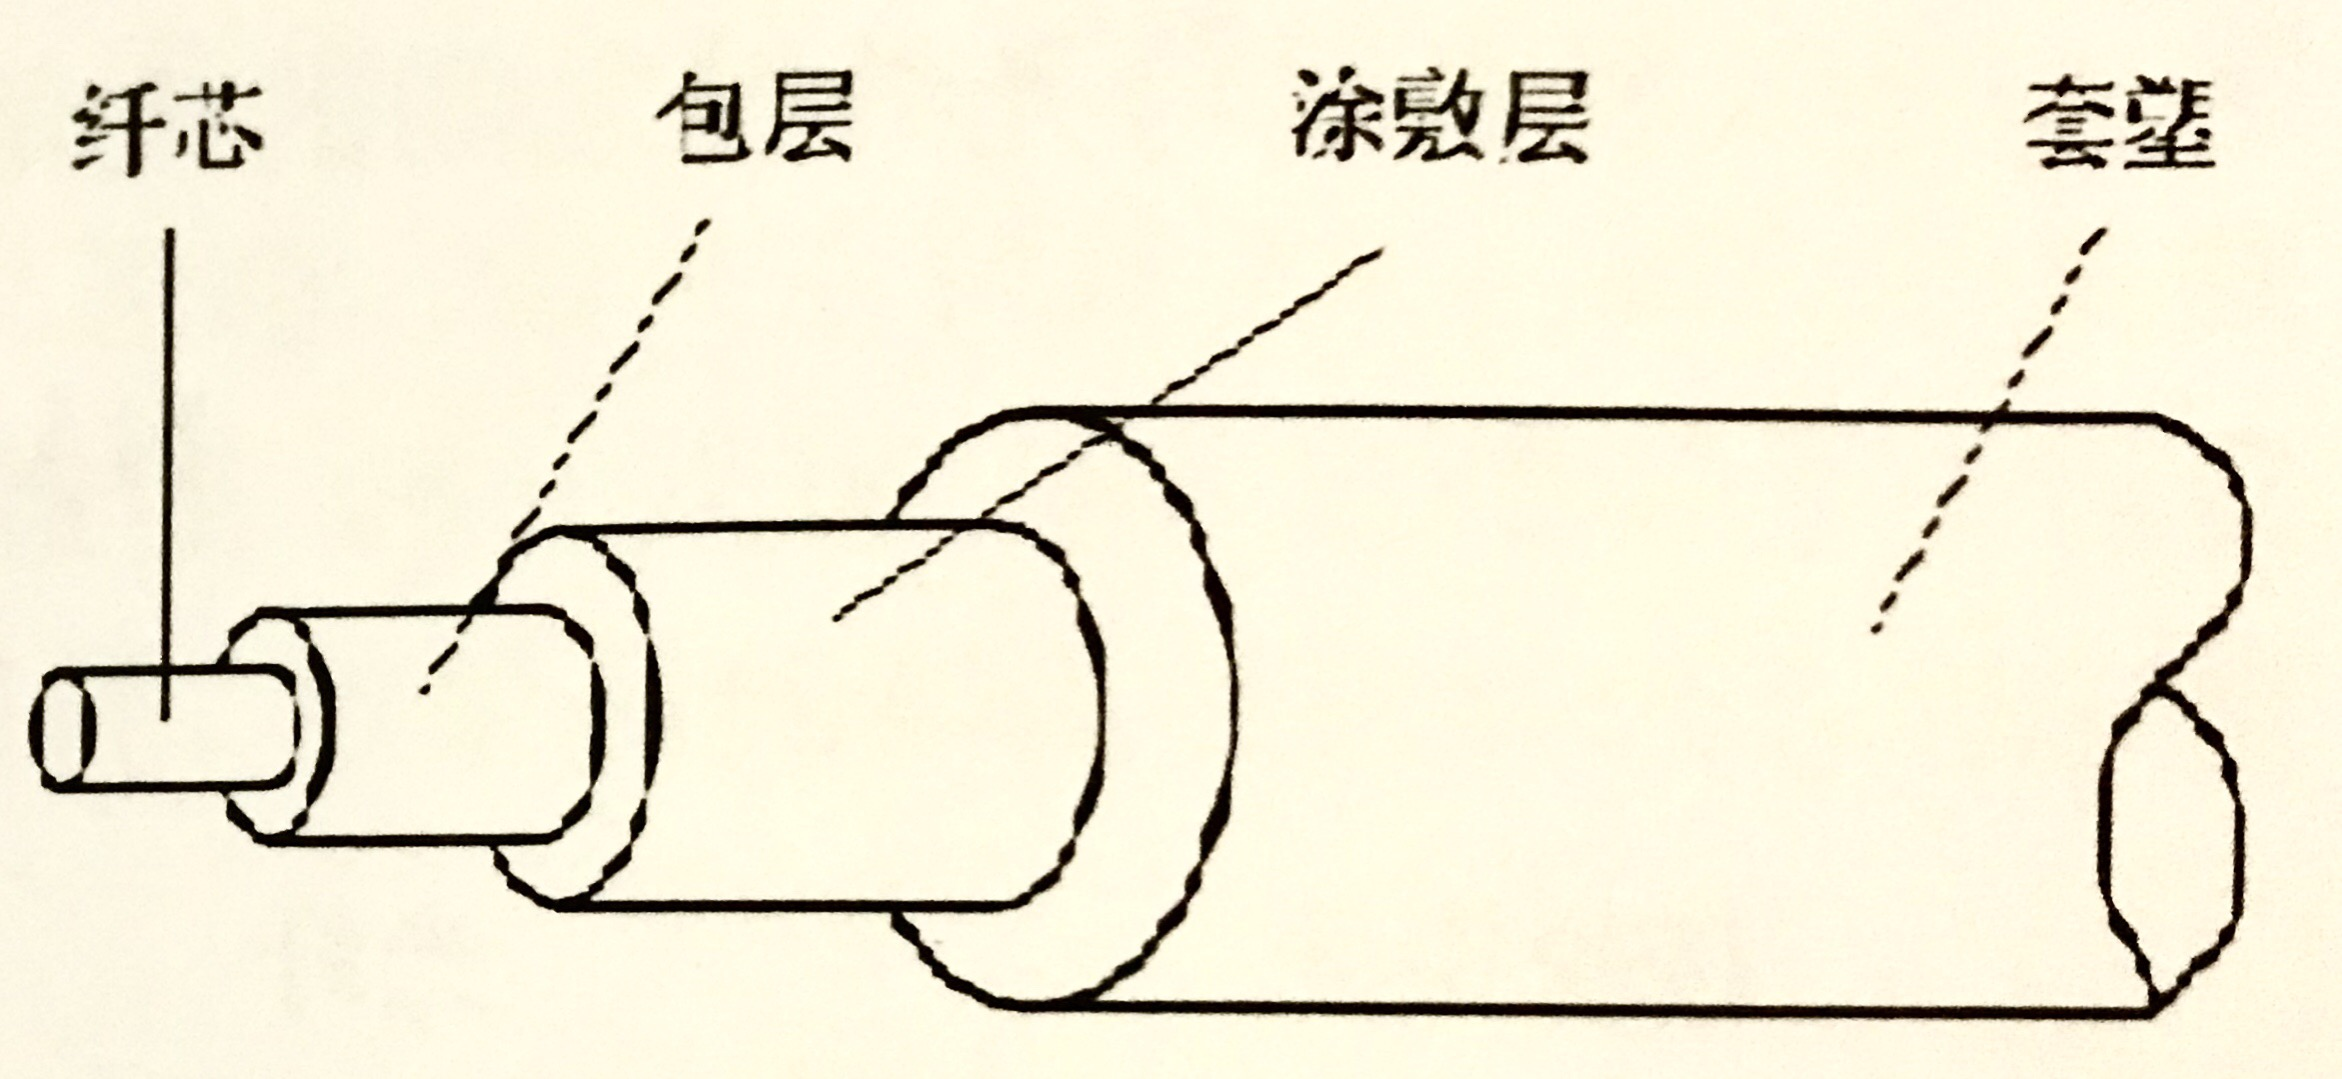
\includegraphics[width=5.5cm]{sturcture}
\caption{光纤结构示意图}
\end{figure}

纤芯一般由直径为$5-50\mu m$、掺有少量$P_2O_5$和$GeO_2$的高纯度$SiO_2$构成,掺杂剂的作用是提高纤芯的折射率。为减少光散射和光吸收,纤芯的杂质含量般不大于$10^{-6}$。

包层主要也是由高纯度$SiO_2$构成,掺有少量的氟和硼以降低其折射率。包层的直径一般为125um。

包层外的涂敷层一般为环氧树脂或硅橡胶,用来增强光纤的机械强度。

光纤的最外层是套塑,套塑大都是采用尼龙或聚乙稀,其作用也是加强光纤的机械强度,没有套塑层的光纤称为裸光纤。

~\\
\noindent\textbf{本实验的目的是:}了解光纤光学的基础知识:学习测量光纤数值孔径和损耗特性的方法;了解光纤温度传感器的工作原理。

\section{实验原理}
\subsection{光源与光纤的耦合效率}
光源与光纤耦合时,为了降低耦合损耗,使更多的光功率注入光纤,获得最大的耦合效率,必须考虑光纤和光源的特性以及具体的耦合方法。He-Ne激光器输出的高斯光束经过透镜后仍为高斯光束。仔细选择透镜的焦距,使经透镜耦合后的高斯光束的束腰(光束中最窄的位置)与纤芯直径相等,即$2W_0=2a$,如图2所示。只要将光纤的端面置于高斯光束的焦点处,即可获得最佳的耦合效率。
\begin{figure}[H]
\centering
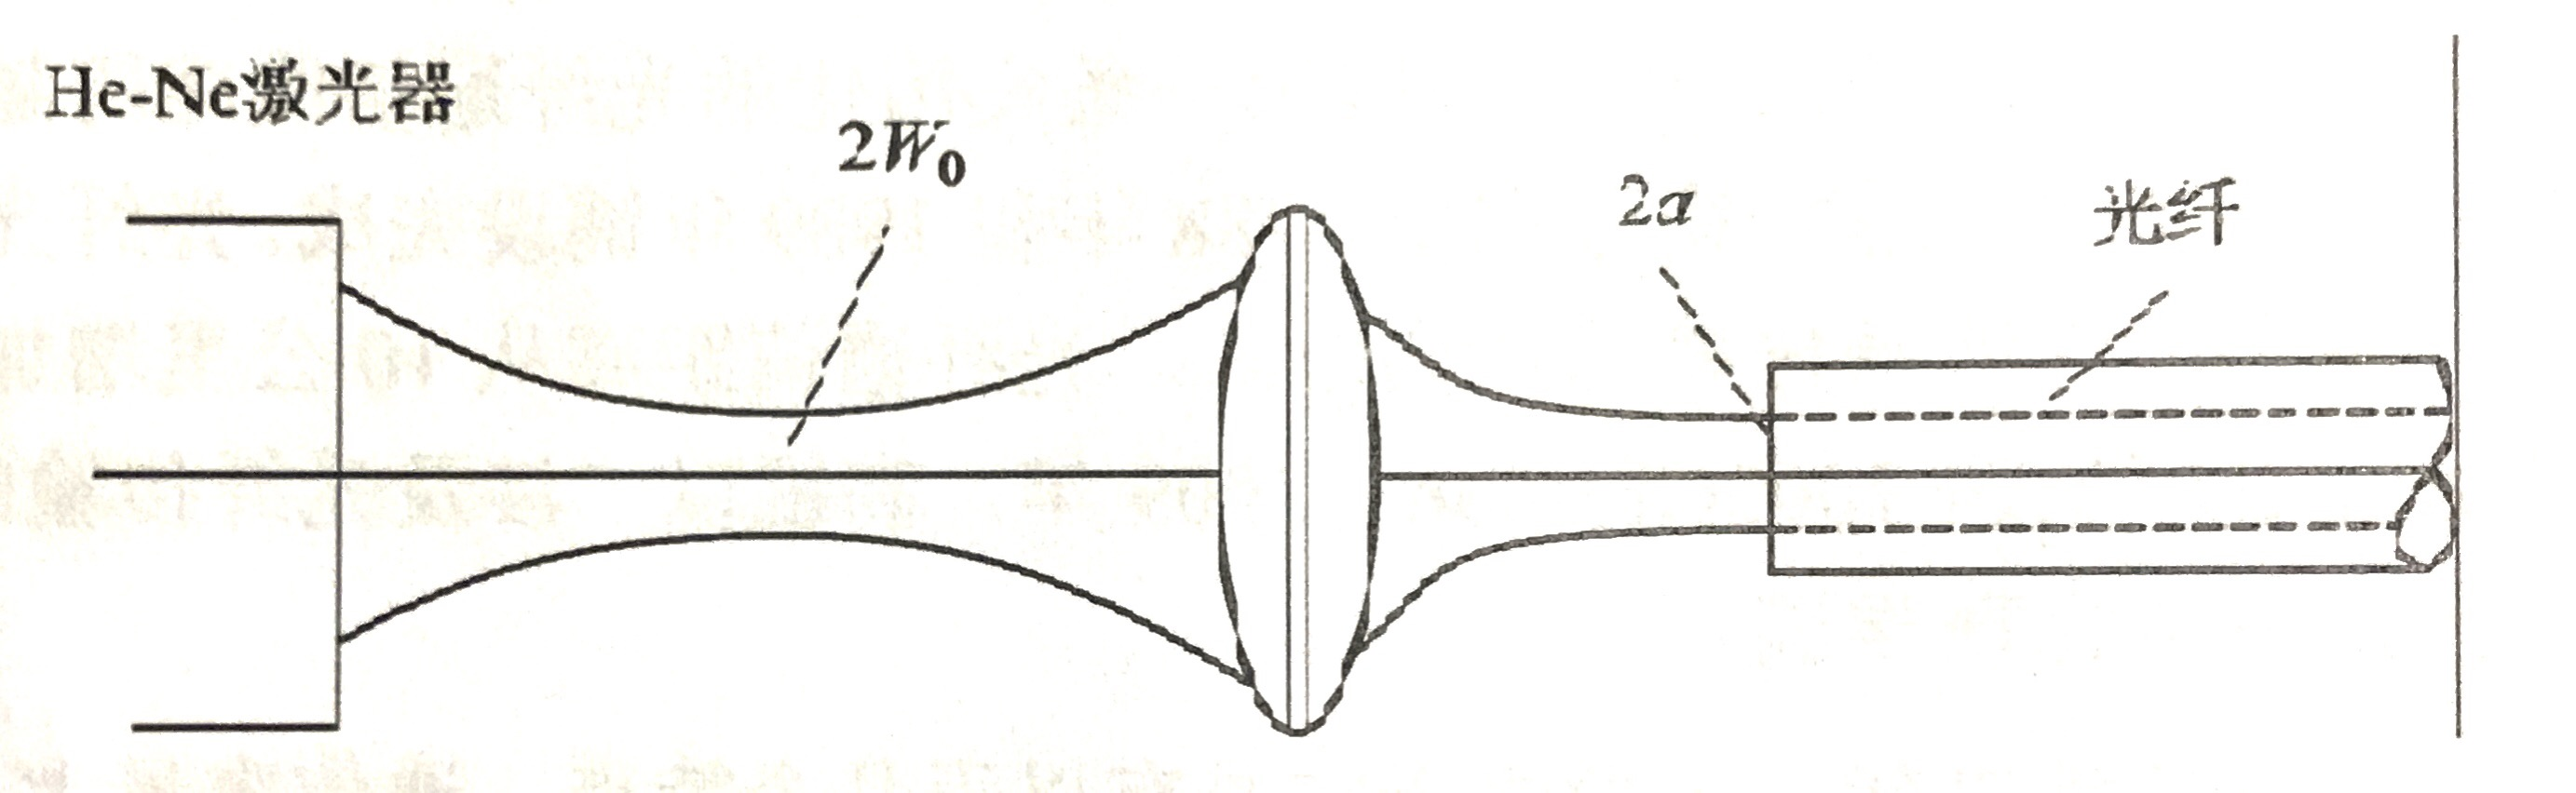
\includegraphics[width=7cm]{interact}
\caption{光纤与He-Ne激光器的耦合}
\end{figure}
耦合效率定义为
\begin{equation}
\gamma=\frac{P}{P_0}
\end{equation}
其中,$P_0$是光纤输入功率,$P$是经光纤耦合后的输出功率。

\subsection{光纤的数值孔径}
光纤的数值孔径(NA-numerical aperture)是表征光纤集光能力的一个重要物理量。由于光线传播具有可逆性,因此,数值孔径既反映了光纤的入射性质,又反映了光纤的出射性质。NA越大,则光纤端面接收或会聚光的能力越强。从几何光学的观点来看,并不是所有入射到光纤端面上的光线都能进入光纤内部进行传播,都能从光纤入射端进去,从出射端出来。而是只有入射角度小于某一个角的光线,オ能在光纤内部传播,如图3所示。
\begin{figure}[H]
\centering
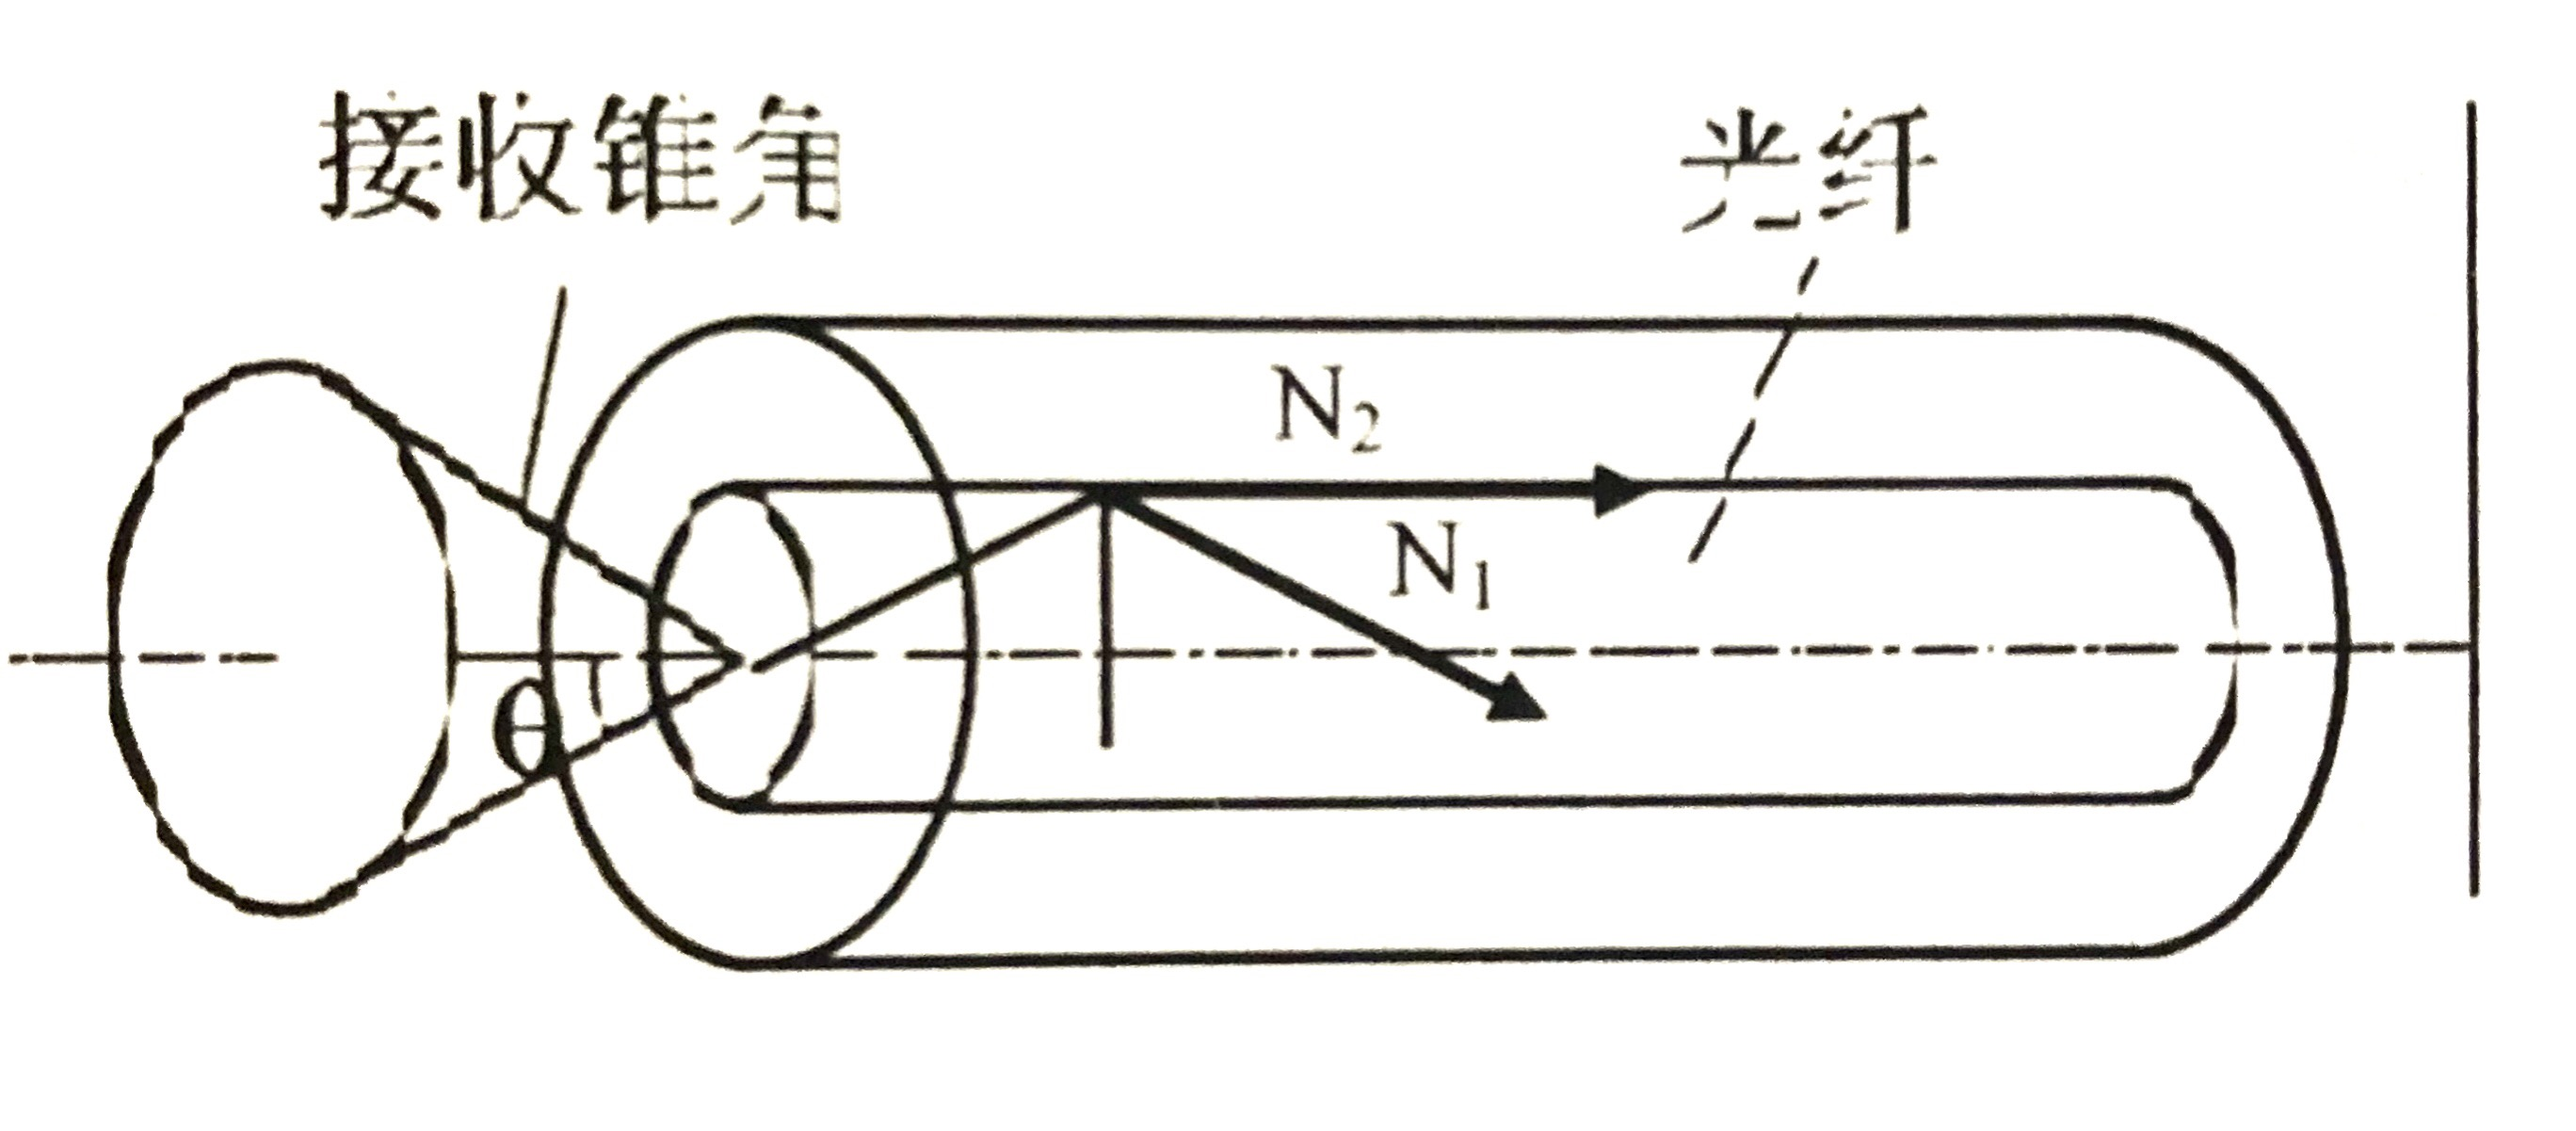
\includegraphics[width=5cm]{NA}
\caption{光纤的数值孔径}
\end{figure}
$\theta$角是入射光线与光纤轴之间的夹角,数值孔径$NA=sin\theta$。

本实验采用“远场光斑法”近似测量光纤的数值孔径,光纤出射的光照射到观察屏上,测出光纤端面与观察屏之间的距离h,以及观察屏上光斑直径2r之后,就可以由下式求出光纤的数值孔径:
\begin{equation}
NA=\frac{n_0}{n_1}sin\theta=\frac{n_0}{n_1}\frac{r}{\sqrt{r^2+h^2}}
\end{equation}
其中$n_0=1$和$n_1=1.464$分别为空气折射率和纤芯折射率。通常情况下包层折射率$n_2=1.460$,则$sin\theta_c=\frac{n_2}{n_1}=0.997$,$NA=sin\theta=0.0739$。

\subsection{光纤的损耗}
光波在光纤中传播会产生各种原因引起的损耗,除接续损耗弯曲损耗等附加损耗外,损耗主要来自于材料的两种固有损耗,一种是瑞利散射引起的,来源于光纤材料结晶的不均匀,其损耗与光波长的四次方成反比;另一种是光纤材料(包含杂质)的吸收,可分为紫外吸收与红外吸收。

光纤对光波产生的衰减作用称为光纤损耗。功率传输损耗是光纤最基本和最重要的特性之一,它在很大程度上决定了光纤通信的中继距离。光波在光纤的实际传输过程中,随着传播距离的增加,光功率以指数形式逐渐衰减,即
\begin{equation}
P(L)=P(0)e^{-\alpha(\lambda)L}
\end{equation}
其中,$P(0)$为光纤的输入功率,$P(L)$为光波传输$L$距离后光纤的输出功率,$\alpha(\lambda)$为损耗系数,
它是光波波长的函数。在光通信中,光信号的损耗一般以分贝(dB)为单位,并采取以下的光纤损耗定义式
\begin{equation}
A(\lambda)=10lg\frac{P(0)}{P(L)}
\end{equation}
损耗系数
\begin{equation}
\alpha(\lambda)=\frac{A(\lambda)}{L}
\end{equation}
本实验采用“截断法”测量光纤的损耗。首先,在稳定的光强输入条件下,测量长度为$L$的整根光纤的输出功率$P_2$;然后,保持耦合条件不变,在离光纤输入端约处截断光纤,测量此短光纤的输出功率$P_1$。当$L\gg l$时,短光纤损耗可以忽略,故可近似认为$P_1$和$P_2$是被截断光纤(长度为$L-l$)的输入功率和输出功率。这样,按照(4)式和(5)式便可以分别求出损耗和损耗系数。本实验所测量的损耗为包括吸收损耗、散射损耗和辐射损耗在内的总损耗。

\subsection{光纤温度传感器}
光纤温度传感器是一种相位调制型光纤传感器,它的工作原理基于光纤双光束干涉相位的变化。由激光器发出的相干光,经光纤分束器分别送入两根长度基本相同的光纤中,其中根叫探测臂,另一根叫参考臂。从两根光纤输出的激光束叠加后将产生干涉,形成干涉条纹。由双光束干涉理论可知,干涉场的光强$I\propto(1+cos)$,$\phi$是相位差,表达式为
\begin{equation}
\phi(T)=\frac{2\pi}{\lambda}n(T)L(T)
\end{equation}
其中,$\lambda$为波长;$n$是光纤折射率,一般为1.458;$L$是光纤的长度;$T$是温度。当$\phi=2k\pi$时($k$为干涉级次),干涉场光强取极大值;当$\phi=(2k+1)\pi$时,干涉场光强取极小值。

当外界的温度作用在其中一根光纤(探测臂)上时,光纤在温度场作用下,长度和折射率都将发生变化,这使得相位也会发生变化$\Delta\phi=\frac{2\pi}{\lambda}(L\Delta n+n\Delta L)$,相位变化将导致干涉条纹产生移动。

\section{实验内容}
\noindent\textbf{1.光源与多模光纤耦合}
\newline(1)打开He-Ne激光电源,预热15分钟。
\newline(2)显微物镜耦合:确定光束通过显微物镜后的焦平面位置,将处理好的光纤置于合适的铜棒中并夹紧,仔细调节五维调整架,使光纤端面处于物镜焦点上;
\newline(3)利用功率计直接测量光源输出功率$P_0$和光纤输出功率$P_1$,计算耦合效率。
\newline\textbf{2.截断法量光纤的损耗特性}
\newline(1)选取约2m长的塑料多模光纤,光纤端面处理后置于铜棒中并夹紧。
\newline(2)当耦合输出功率最大时,用功率计测量此时的功率值$P_1$。
\newline(3)在距光纤输入端约10cm处剪断光纤,并测量截下长光纤的长度$L$,测量此时的输出功率值$P_2$;计算光纤的损耗和损耗系数。
\newline\textbf{3.光纤的数值孔径测量}
\newline 根据远场光斑法的定义,设计并测量单模光纤的数值孔径。
\newline\textbf{4.温度传感器}
\newline(1)用步骤3的光纤作为温度传感器的输入光纤,使其耦合最佳。
\newline(2)处理光纤温度传感器的两根输出光纤,仔细调节它们的位置和间距,并调节监视器的位置直到观察到干涉条纹。
\newline(3)缓慢调节一根光纤上的温度,观察干涉条纹的移动,确定其条纹变化数和温度之间的关系。

\section{实验结果分析与讨论}
\noindent\textbf{1.塑料光纤参数测量}
\begin{figure}[H]
\centering
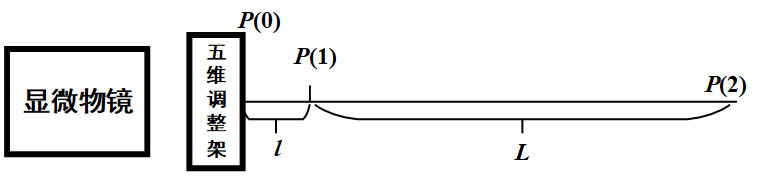
\includegraphics[width=7cm]{p}
\caption{塑料光纤的测量}
\end{figure}
如图4,塑料光纤截断前测得的输出功率$P_2=0.704mW$;截断长度$L=124.20cm$,截断后剩下部分的长度$l=9.24cm$,远小于$L$,故截断后测得的输出功率$P_11.245mW$可看作经光纤耦合后的输出功率。计算得光纤损耗$A(\lambda)=10lg\frac{P_1}{P_2}=2.48$,损耗系数$\alpha(\lambda)=\frac{A(\lambda)}{L}=1.99$。

测得光源输出功率$P_0=2.74mW$,计算得耦合效率$\gamma=\frac{P_1}{P_0}=45.4\%$。

~\\
\noindent\textbf{2.单模G625光纤参数测量}

由于长度较短,商用光纤的传输损耗可以忽略,可将输出功率$P_1=0.502mW$看作经光纤耦合后的输出功率;光源输出功率$P_0=2.74mW$,计算得耦合效率$\gamma=\frac{P_1}{P_0}=18.3\%$。可见塑料光纤的耦合效率较高,商用光纤的耦合效率较低,主要是由于二者的导光部分的半径塑料光纤大于商用光纤,可进入的光较多。
\begin{figure}[H]
\centering
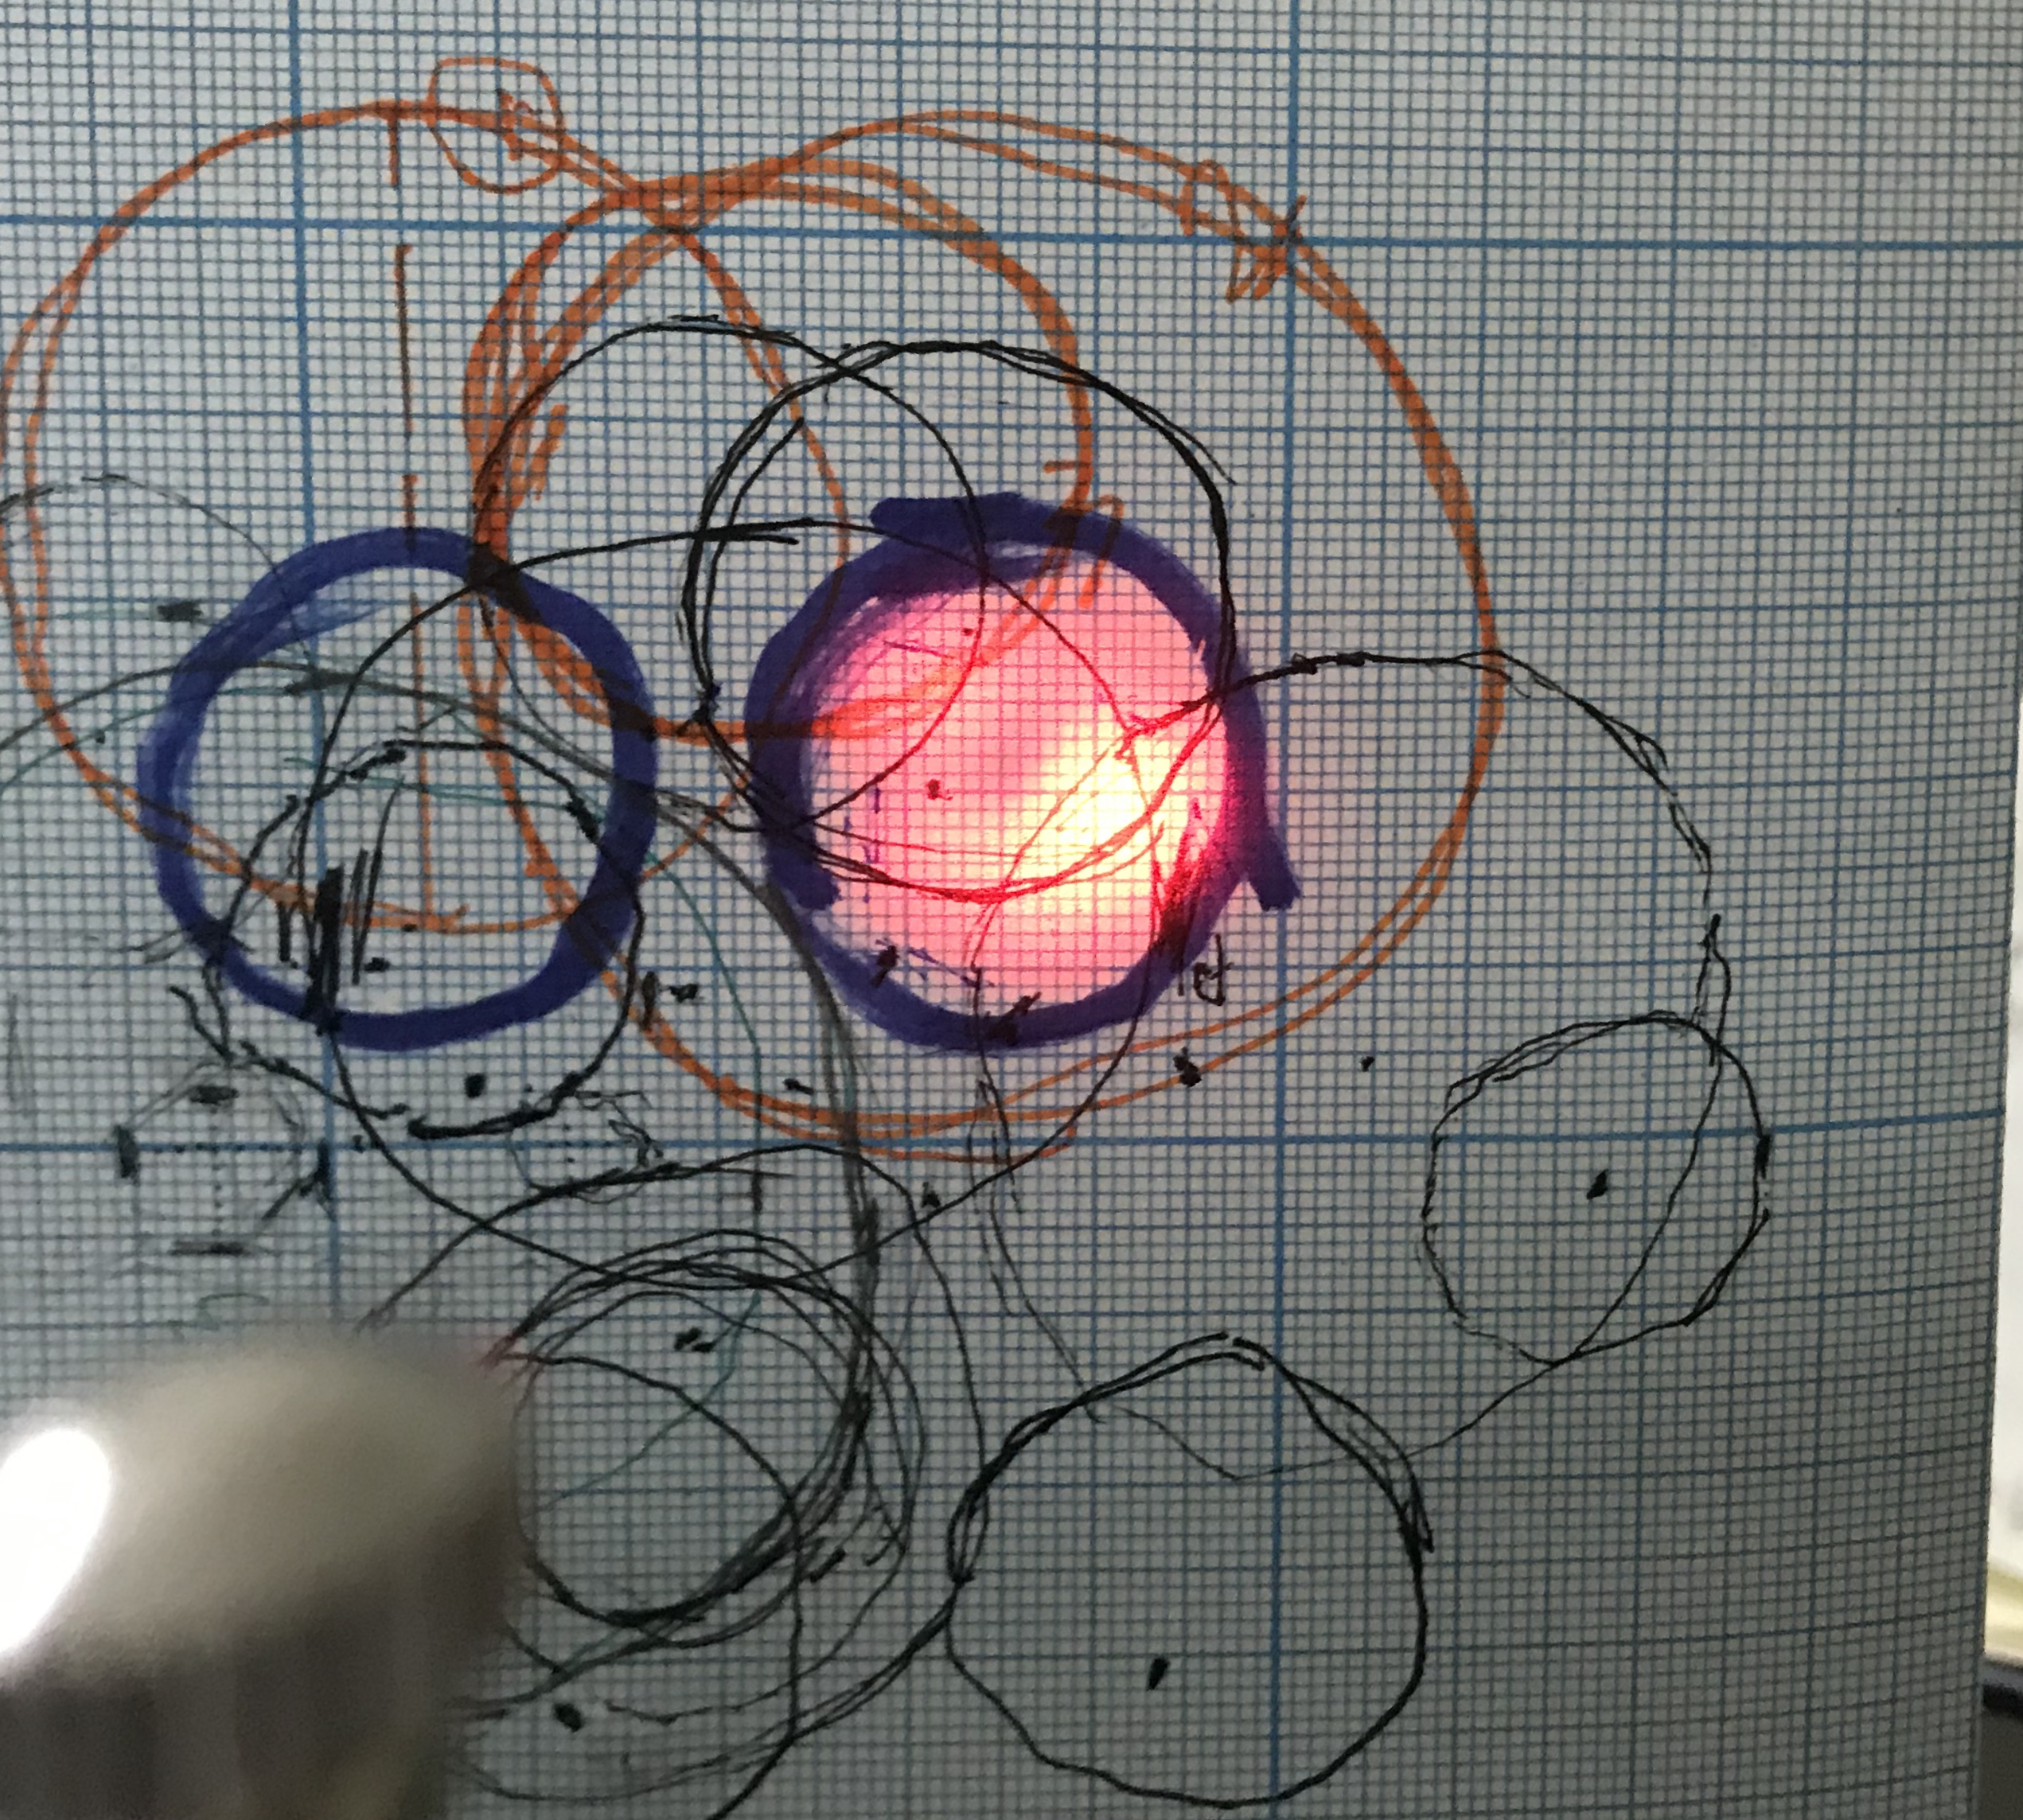
\includegraphics[width=4cm]{single}
\caption{光斑形状}
\end{figure}
如图为远场光斑法测量得到的光斑,测得光斑半径$r=1.12cm$,出光口到光屏的距离$h=10.32cm$,数值孔径$NA=\frac{n_0}{n_1}\frac{r}{\sqrt{r^2+h^2}}=0.0737$;理论值$NA=0.0739$,测量误差为$0.24\%$。

~\\
\noindent\textbf{3.温度传感器}

做该实验时,观察到随着加温器温度上升,干涉条纹移动。升温时移动较为稳定;而降温时在温度较高时容易出现回缩现象,温度降低后移动较为稳定。

主要原因是实验操作时并没有使对照边的传导线远离升温器,升温器在高温下对对照边的加热现象较为严重。
\begin{figure}[H]
\centering
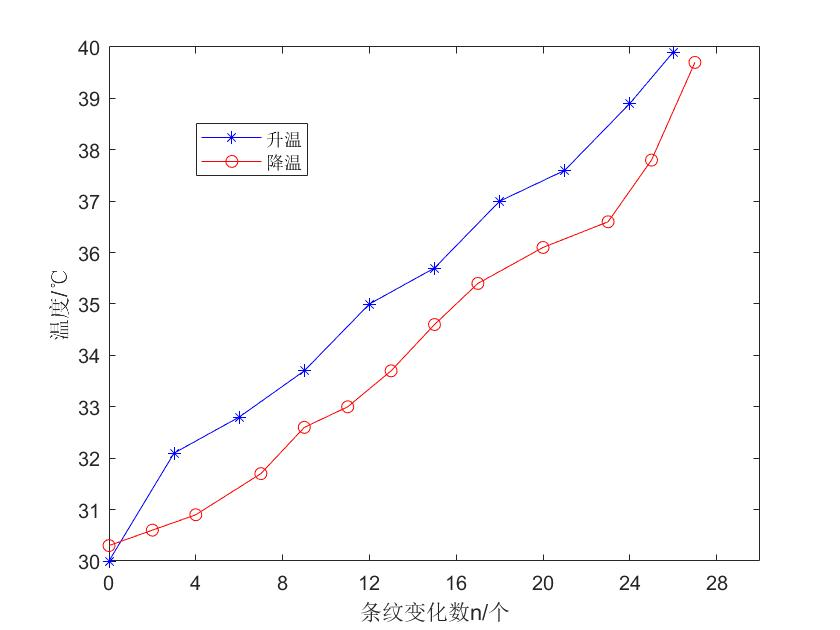
\includegraphics[width=8cm]{thermal}
\caption{干涉条纹变化数-温差曲线}
\end{figure}
如图6为升温和降温分别测得的干涉条纹变化数-温差曲线,可见:

(1)两条曲线都不呈现出线性,这是由于温度改变时,引起条纹移动的主要原因是纤芯材料的折射率的改变,而纤芯材料折射率与温度的变化关系并不呈线性;

(2)两条曲线并不重合,是由于温度改变时会引起纤芯长度变化,长度变化也会引起两束光的相位差,升温和降温时对应的长度应变并不相同。

\section{误差分析}
\noindent 1.测量数值孔径时,手动测量出光口到光屏距离,可能存在一定误差;另外光斑并不是准确的圆形,且边缘分辨率较低,因此测量光斑半径时可能存在一定误差。
\newline 2.做温度传感器实验时并没有使对照边的传导线远离升温器,使测得的条纹变化并不对应真实的温度差造成的条纹变化数,存在一定误差。

\section{结论}
实验测量了塑料光纤的损耗特性、商用光纤的数值孔径和二者的耦合效率,其中塑料光纤的耦合效率较高,商用光纤的耦合效率较低,主要是由于二者的导光部分的半径塑料光纤大于商用光纤,可进入的光较多;

而后利用光纤作为温度传感器,观察到了温度变化时,两束光相位差引起的干涉条纹移动,测量了干涉条纹变化数和温度之间的关系,得到了变化数-温差曲线,可见虽说温度变化可以由导光材料随温度变化折射率的变化函数得到,但是影响光纤温度传感器分辨率的还有温度引起的光纤长度变化,要利用光纤温度传感器标定温度需要测量升温和降温两次的温度。

\section{参考文献}
\small
\noindent[1]北师大物理实验教学中心,近代物理实验2讲义p72-80,2019.

\end{multicols}

~\\
\begin{figure}[htbp]
\subfigure{
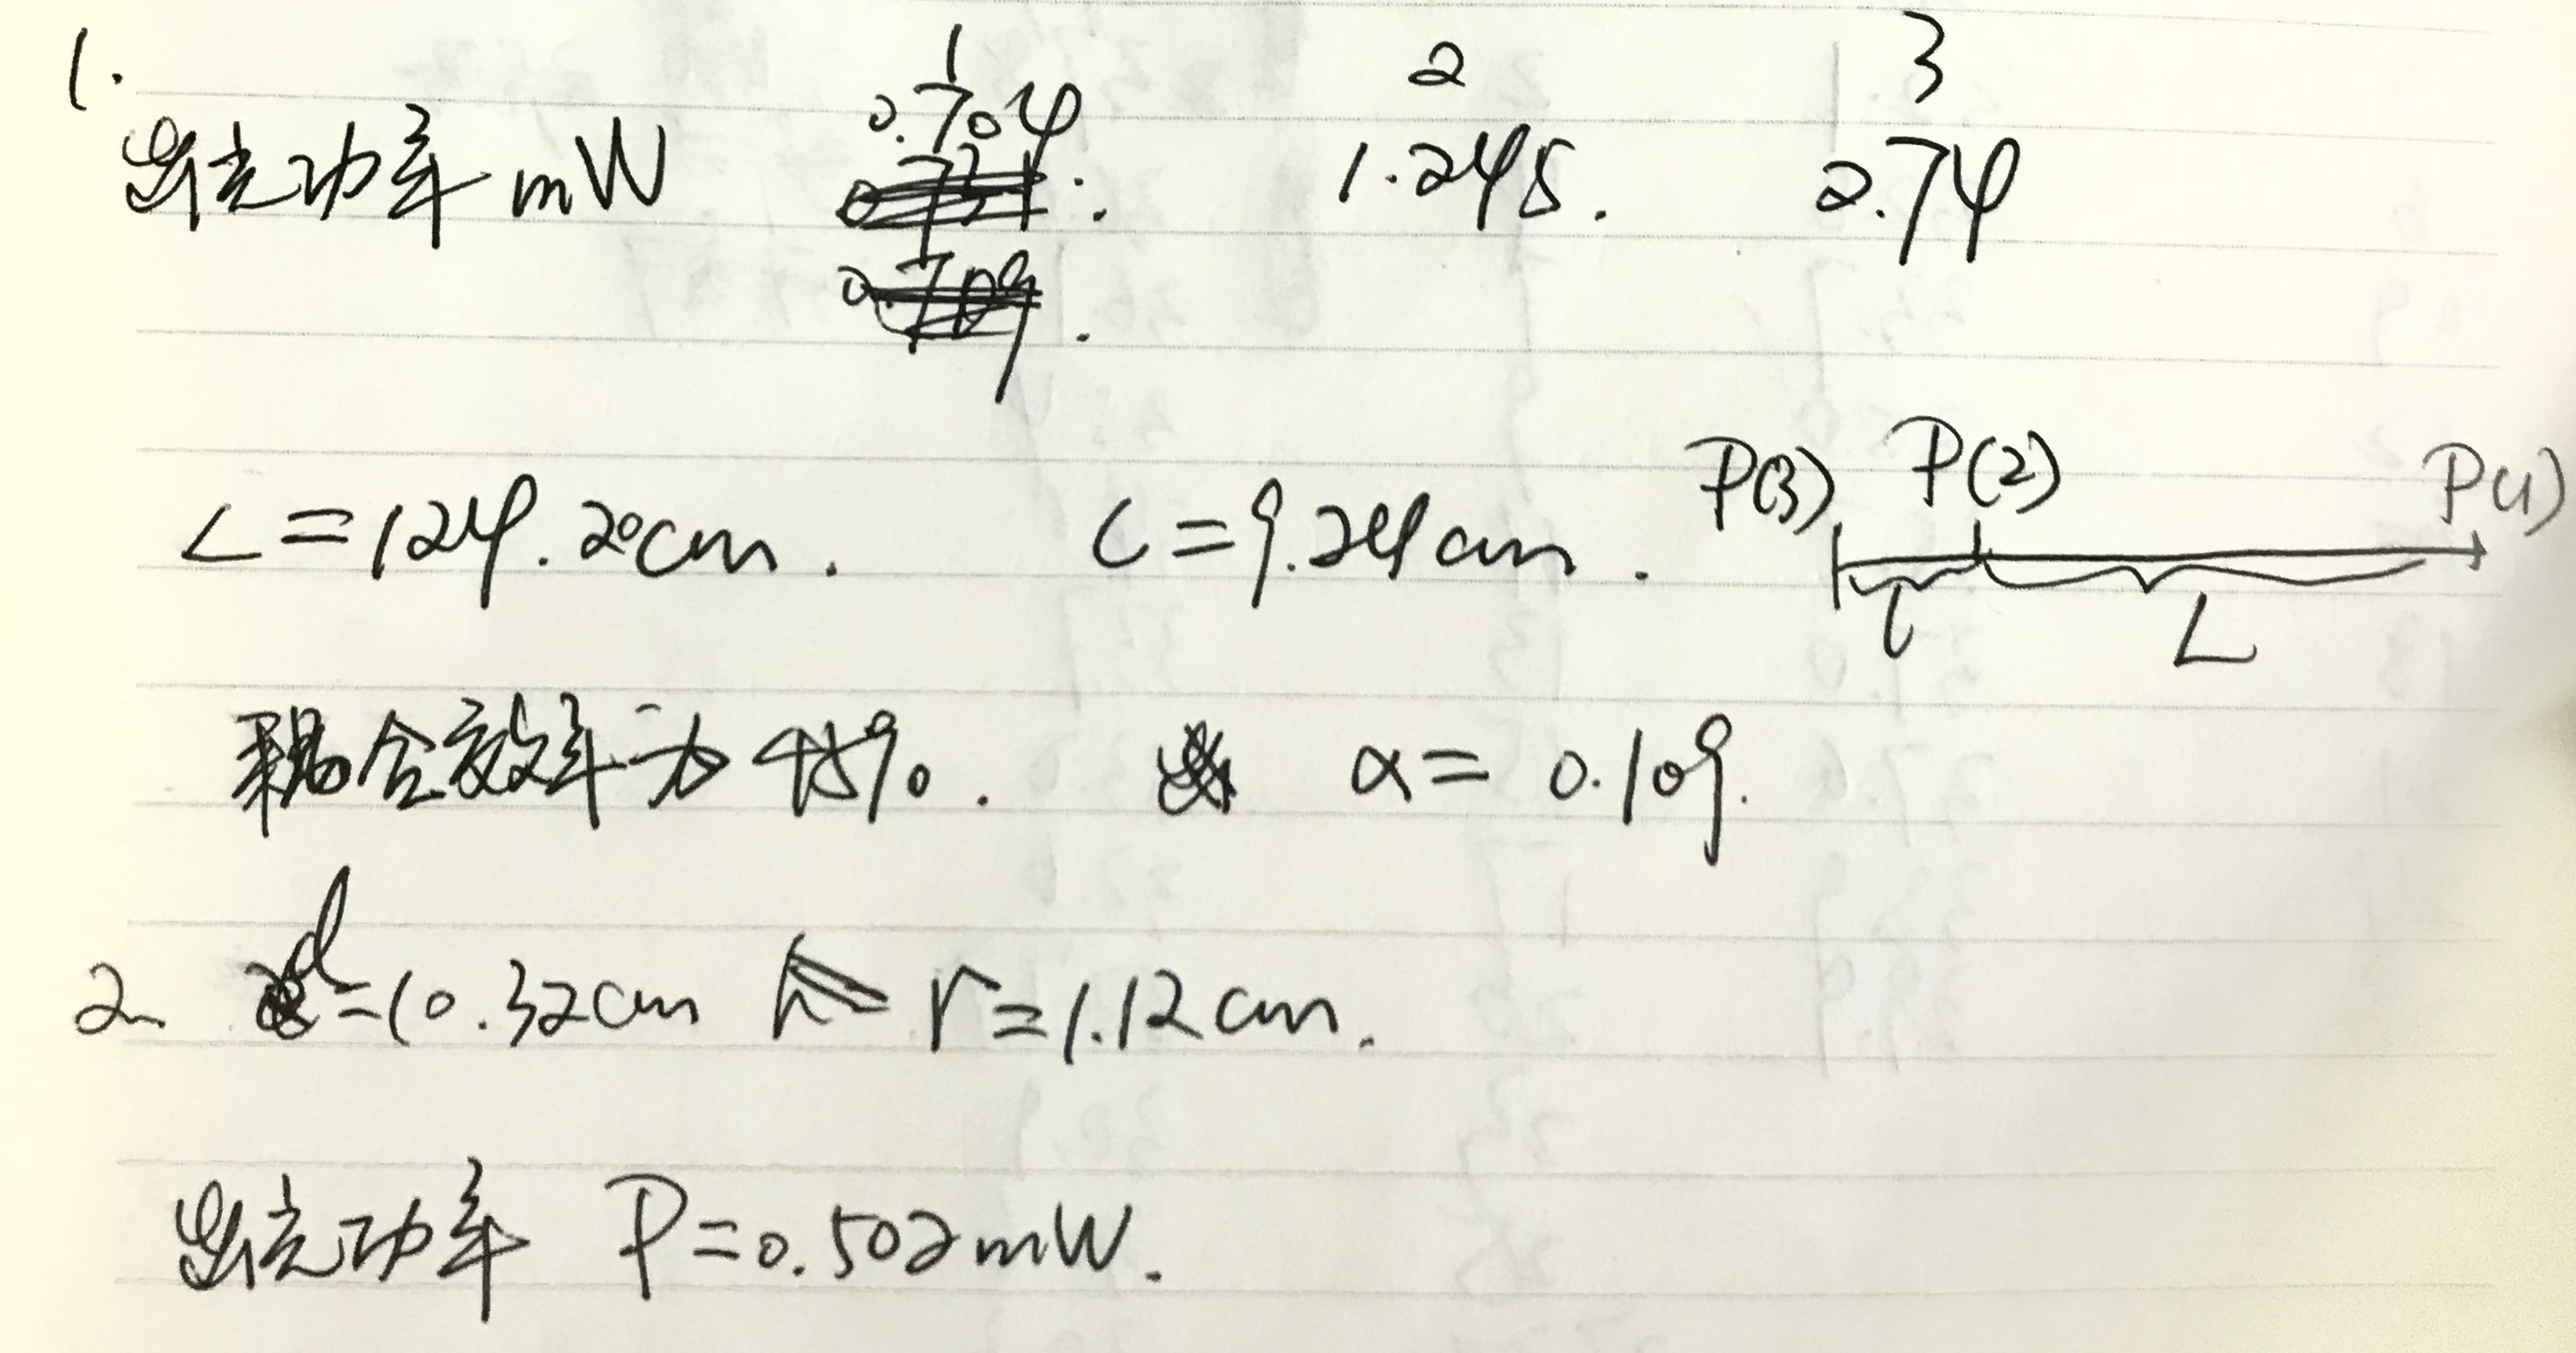
\includegraphics[width=8.5cm]{s1}
}
\subfigure{
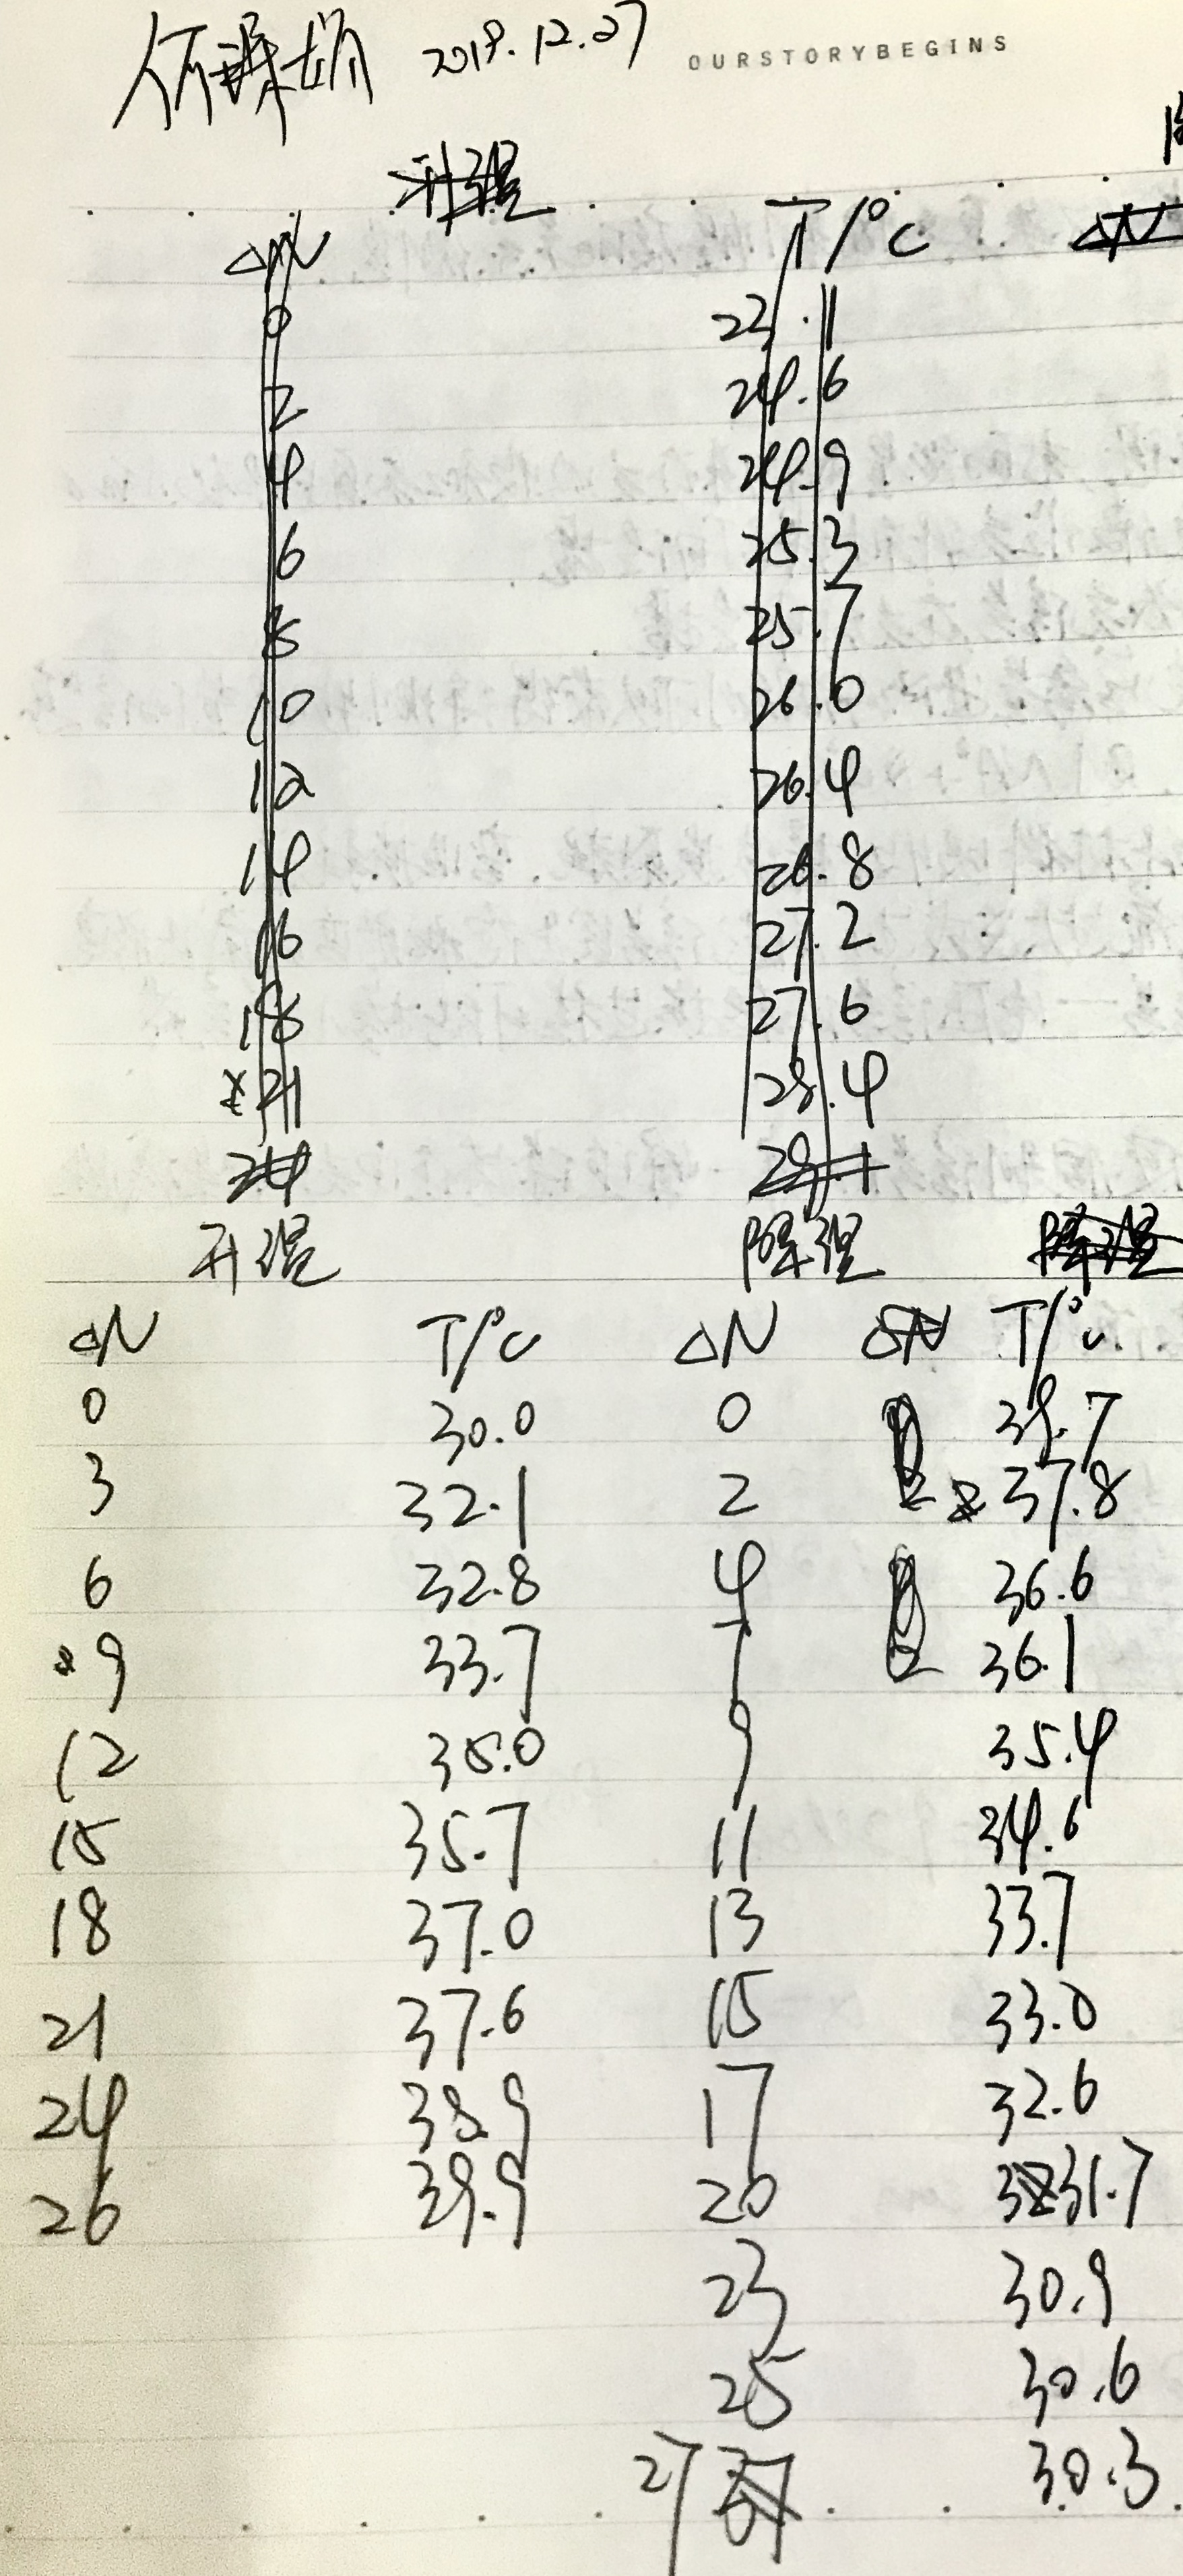
\includegraphics[width=6cm]{s2}
}
\end{figure}


\end{document}